% TODO:
%  Add a bit more detail about detectors in the HMS hut
%  Table of SHMS performance specifications in SHMS section
%  HMS window details in ``Vacuum Windows in Hall C'' table
% Check the statement:
%    The HMS entrance window is located near the pivot and has a center-to-center
%   bolt hole diameter of $10.5$ inches.


\infoleveqnull{\section{Hall C Spectrometers}}
%\section{Introduction}

	The two magnetic spectrometers in Hall~C are designed to perform
high resolution and high accuracy nuclear physics experiments.  These
spectrometers transport and detect charged particles that are scattered or produced 
in beam-target interactions.
\infolevone{
In this chapter
we discuss the features and safe operation of these spectrometers,
the High Momentum Spectrometer, or HMS,
and Super High Momentum Spectrometer, or SHMS.  These spectrometers
share many common features.  After this
introduction and overviews of the individual spectrometers, the
spectrometers are discussed together as a series of subsystems.
This chapter covers the ``mechanical'' subsystems of the spectrometers.
The detector packages and
shield houses are discussed in Chapter~\ref{chap:detectors}.

Both the HMS and the SHMS are designed around a series of superconducting magnets,
including quadrupoles and dipoles, followed by a set of particle detectors.  The first
magnet on the SHMS is a horizontal-bending (HB) dipole that bends particles
away from the beam-line. The HMS does not have a horizontal bender.
The primary purpose of the quadrupole magnets is to increase the flux of
charged particles entering the main dipole magnets and to focus the orbits of the
charged particles into the detector huts.
The dipole magnets deflect charged particles vertically
as they enter the detector huts. Some of the detectors measure the amount of deflection
so that we may
determine the momentum of each particle. Other detectors provide accurate timing 
to trigger the readout of all detector data, or they measure a particle's speed
or total energy so that we can determine its mass.

Each spectrometer is built on a rotatable support structure or ``carriage". 
These ride on steel 
wheels and rails and rotate around the pivot. Experiments using the HMS or
SHMS place their experimental targets along the beamline above the pivot.
The support structures carry the weight of the magnets and detectors, and keep
them aligned to one-another and pointed at the target. On the SHMS, the shield 
house and all of the
other spectrometer equipment are also carried by the support structure. The
HMS has a separate carriage that supports the weight of the shield house.

During beam operations a many particles are scattered and
produced in the target. A few of these enter one of the spectrometers. Most of 
them go forward at small angles and are stopped in the beam dump. The
remainder, scattered over a wide range of angles,  interact with the beam pipe, 
the air, nearby structures, etc., and
constitute background radiation that would overwhelm the detectors.
The shield houses have thick walls that are designed to reduce the amount of
radiation that gets inside. Both spectrometers use
concrete and lead lining on the walls as shielding. On
the SHMS, two custom types of concrete improve the neutron stopping power 
of the walls by
adding boron (in the form of boron-carbide) or extra hydrogen (recycled
plastic chips). Each shield house has a room that surrounds the detectors.
The SHMS has a second room, shielded from the first, that protects the
electronics of the DAQ system and the magnet control systems.

%Each spectrometer includes a shield house which contain the particle
%detector packages.  In the case of the SHMS, this shield house (and a separate
%shield house for electronics) are part of the carriage structure.  In
%the case of the HMS, the detector shield house is a separate
%structure, coupled to the carriage by a ``push bar'' on the ``pasta fork''.
%The ``pasta fork" is the name given to the steel piece that protrudes
%from the back of the carriage. The detector frame is supported on the
%``pasta fork." This insures that the detectors do not move relative
%to the magnetic elements.

\section{High Momentum Spectrometer (HMS) }

The HMS, which operates on the beam-right side of the beamline, 
includes three superconducting quadrupole magnets and one superconducting dipole magnet. The quadrupoles were
manufactured for JLab by {\em OXFORD} while the dipole was built for
JLab by {\em ELIN}.  The quadrupole magnets are referred to as Q1, Q2,
and Q3, where a particle first traverses Q1, then Q2 and Q3, and
finally traverses the dipole magnet. The dipole of the HMS deflects central-momentum
particle trajectories upwards by $25^{\circ}$.


The magnet system is followed by a large concrete detector hut, in which all
detector elements reside. The main fraction of the detector elements have been
built by universities involved in the Hall~C physics program.  These
detectors are described in chapter~\ref{chap:detectors}.

The HMS spectrometer can be moved to scattering angles between
$10.5^{\circ}$ and $90^{\circ}$. This range is usually constrained by
administrative, software and hardware limits depending on what
downstream beam pipe is installed and what obstructions are currently in the hall.  The
maximum momentum accessible to the HMS magnet
system is presently $6~\textrm{GeV}/c$. This limit is expected to increase
once the HMS dipole has been certified for use at higher momenta during 
the 12 GeV era.

\section{The Super High Momentum Spectrometer (SHMS)}

The Super High Momentum Spectrometer (SHMS) operates on the beam-left
side of the beamline, and can be rotated around the pivot for scattering angles from 5.5
to 40~degrees. It was built between 2009 and 2016 as the major
Hall-C component of the 12-GeV Upgrade Project.  The five superconducting
magnets on the SHMS can be set for a central-ray momentum of up to 11~GeV/c.
The minimum design momentum is 2 GeV/c. A CAD model of the SHMS is shown
in Fig.~\ref{fig:SHMS_CAD_Model}, and Table~\ref{tab:shms_specs} lists the performance specifications. 

\begin{figure}
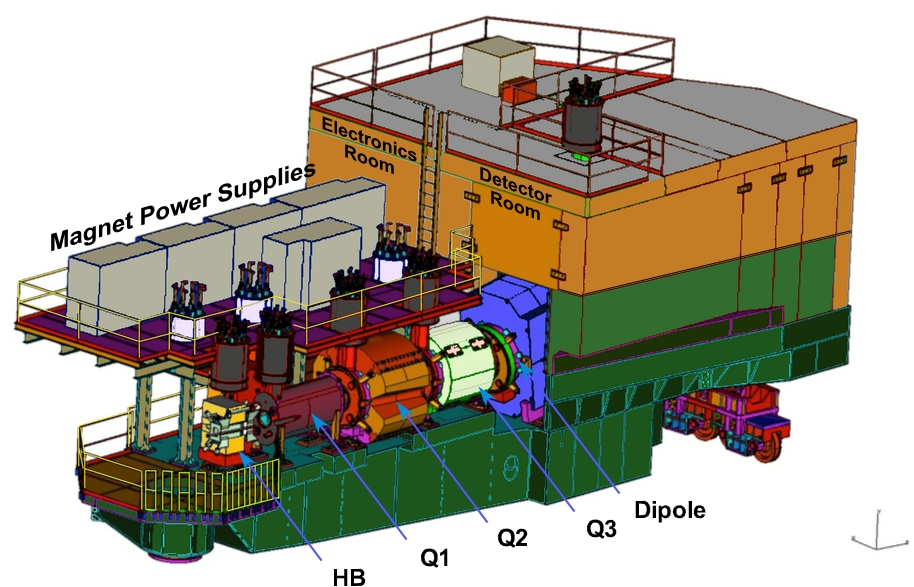
\includegraphics[width=6in]{SHMS_Rendered_Recolored_Annotated}
\caption{CAD Rendering of the Super-High-Momentum Spectrometer. \label{fig:SHMS_CAD_Model}}
\end{figure}

\begin{table}
\begin{center}
\caption{SHMS Design Parameters\label{tab:shms_specs}}
\vspace{\baselineskip}
\begin{tabular}{|l|l|} 
\hline
Parameter						& SHMS Design 			\\ \hline
Range of Central Momentum		& 2 to 11 GeV/c for all angles	\\
Momentum Acceptance $\delta$	& $-10\%$ to $+22\%$			\\
Scattering Angle Range			& 5.5 to 40 degrees			\\
Solid Angle Acceptance			& $>$ 4.0 millisterradians		\\
Horizontal Angle Resolution		& 0.5 - 1.2 mrad			\\
Vertical Angle Resolution			& 0.3 - 1.1 mrad			\\
Vertex Length Resolution			& 0.1 - 0.3 cm				\\
Tracking Rate Capability			& 5 MHz					\\
Beam Capability				& Up to $90 \mu$A			\\
\hline
\end{tabular}
\end{center}
\end{table}


The primary magnetic elements on the SHMS, the Q1, Q2, Q3, and Dipole magnets, provide
point-to-point focusing and momentum dispersion just like the four magnets with
the same names on the HMS. The dipole of the SHMS bends central-momentum particles
trajectories up by $18.2^{\circ}$. The SHMS Q1 was 
manufactured by Scientific Magnetics, Inc. in Abingdon, England. Q2, Q3, and
the Dipole were constructed by Sigmaphi in Vannes, France.

In order to reach the smallest scattering angles, the SHMS has a horizontally-bending dipole
magnet as its first magnetic element. Referred to as ``HB", it was built by FRIB, the Department of Energy
facility at Michigan State  University. This small, high-field magnet bends
central-momentum particles to the left by 3~degrees so that the remainder of the
spectrometer parts will be further away from the primary electron beam. The HB
magnet is an asymmetric ``C''-dipole which has a flux-return iron yoke only on
the side away from the primary beam. When the SHMS is set for small scattering 
angles, the electron beam passes very close to the spectrometer and to the
HB magnet's superconducting
coils. In this configuration the coils see a high radiation dose which may cause
them to have a limited 
lifetime. Experiments must be planned in such a way that this exposure is minimized.

A further consequence of making the SHMS operate at small scattering angles is
that the iron yokes of the HB and Q2 magnets had to be designed with notches 
that just clear the beamline vacuum pipe. The fringe fields from these magnets can
deflect the primary electron beam away from the middle of the beam dump. 
The effects of this field
must be mitigated by a combination of good experiment planning, magnetic shielding, 
and automatic safety systems.

The SHMS shield house has two rooms. The dipole magnet penetrates the front
wall of the room containing the detectors. Inside this are the two sets of 6-plane
drift chambers, the Heavy-Gas Cerenkov (HGC), the two pairs of trigger hodoscopes 
(S1X/S1Y and S2X/Q2Y), and
the Preshower and Shower Counters (calorimeters). The SHMS focal plane forms an 
angle of about 5~degrees with respect to the central trajectory, 
and intersects that trajectory at
a point midway between the two drift chamber boxes. Additional  particle-identification
detectors (Noble-Gas Cerenkov (NGC), and/or Aerogel Cerenkov) may also be 
installed if needed by the current experiment. When the NGC is not in use it may
be replaced by a tank that extends the vacuum system up  to a window just in
front of the first drift chamber. In this configuration, a mechanical safety shutter
must be closed over this large vacuum window before personnel may enter the
room.

The second room in the SHMS shield house houses the
electronics controlling the magnet power supplies, the data-acquisition 
electronics (DAQ) and power supplies for the detectors, and theVESDA
smoke and flammable gas sensor systems. When personnel enter the shield
house they first pass into this "Electronics Room". 
}

\begin{safetyen}{0}{0}
\infolevone{\section{Safety Information}}
\label{sec:spectrometer-safety}

\subsection{Hazards}

The spectrometers have associated vacuum, electrical, cryogenic and
magnet systems all of which can be extremely dangerous due to the size
and stored energy in the systems.  
Parts of the spectrometers are at elevated levels which would present fall
hazards if the installed safety equipment were not present.
Hazards of rotating the
spectrometers as well as the particle detectors that get placed inside
the detector hut of the spectrometer are covered in detail in
following sections.

Signage and alerts are placed to remind workers of some of the potential hazards
in Hall C, but each individual is ultimately responsible for his or her own 
safety. Always read and respect warning signs, and never attempt to 
circumvent barriers or other equipment
that has been installed for your protection. If you discover what appears to be a
new or unidentified hazard, protect your coworkers by warning them
and alert the Hall-C management and Safety Warden.

\subsection{Mitigations}

Both of the spectrometers have elevated work platforms that are secured by
gates and handrails. Never attempt to bypass these protections. During experiment
running periods, in order to allow spectrometer rotation, it may be necessary to
remove the handrails around the target platform. In this condition access to the 
target platform is restricted to trained individuals who have been specifically
authorized to work near there. Fall-protection equipment is required.

The vacuum systems associated with the spectrometers are essentially 
pressure vessels and care should be exercised so as not to damage or puncture the 
vacuum windows.   The large vacuum windows inside the two shield houses are protected
by shutters which must be lowered into place before the access door to the
detector rooms will open. (When the Noble-Gas Cerenkov (NGC) is installed in the SHMS, 
the NGC itself protects the vacuum window and the shutter is not present.)
During hall maintenance, covers are placed over the spectrometer
vacuum windows near the pivot to help prevent anything from accidentally hitting 
a window. Hearing protection may be required when you work near a vulnerable
vacuum window. As conditions may change, please take note of currently posted
warning signs and instructions.

The magnets themselves are installed inside cryostats.  These vessels 
are exposed to high pressures and are therefore equipped with safety 
relief valves and burst discs.   

The cryogenic system operates at an elevated pressure and at temperatures
about 4~Kelvin (helium system) and about 90~Kelvin (nitrogen system).  One must
guard against cold burns and take the normal precautions with pressure
vessels when operating or working near this system.  Manipulation of any cryogenic 
system component such as a U-Tube or manual valve may only be performed by
a trained cryogenic-system expert.

When they are powered, the magnets have a great deal of stored energy as they are large 
inductors. (See Table~\ref{tab:magnet_parameters}.) Always make sure people are clear of 
the magnets and their dump resistors.

\subsection{Responsible Personnel}

In the event that problems arise during 
operation of the spectrometers, qualified personnel should be notified
(see Table \ref{tab:spec:personnel_technical}).  
This includes any prolonged or serious problem with the source of magnet 
cryogens (the ESR).  (See also "Checking Cryogenics" in Section \ref{ssec:operatemagnets}, below.)
On weekends and after hours there will be a 
designated individual on call for magnet services.  Any member of the 
Hall C technical staff is qualified to deal with unusual magnet 
situations but in the event of serious problems the person on
call should be contacted.

\begin{namestab}{tab:spec:personnel_technical}{Spectrometers: authorized personnel}{%
      List of spectrometer responsible personnel where ``W.B.'' stands for the white board 
      in the counting house.}
   \TechonCall{\em Contact}
   \PaulBrindza{}
   \SteveLassiter{}
   \EricSun{}
   \MikeFowler{}
   \JoeBeaufait{}
   \JackSegal{}
   \MahlonLong{}
\end{namestab}


\end{safetyen}

\infolevone{
\section{Features Common to Both Spectrometers}

\subsection{Vacuum Windows}

Because multiple scattering degrades the performance of a spectrometer, it is
important that the spectrometer volume be evacuated and that the vacuum
entrance and exit windows be as low mass as possible. However,
catastrophic window failure would generate a significant shock wave as air
rushed to fill the vacuum volume. It would also cause a loud noise which
could cause hearing damage to anyone in the immediate vicinity.
The material chosen for the vacuum windows, then, must be both light enough
to have a minimum effect on the beam and strong enough to operate reliably and safely.

{\bf One of the responsible personnel must be present for
any work directly affecting any Hall~C vacuum window}. Refer to Table ~\ref{tab:spectrometers:personnel_vacuum}.

Thin metal windows have an indefinite lifetime and cause
multiple scattering which is small compared to the intrinsic resolution of
the Hall-C spectrometers. Both the HMS and the SHMS are now equipped
with metal windows, as detailed in Table ~\ref{tab:hall_c_windows_specs}.

\begin{namestab}{tab:spectrometers:personnel_vacuum}{Spectrometer Vacuum: authorized personnel}{%
      List of Spectrometer Vacuum responsible personnel where ``W.B.'' stands for the white board 
      in the counting house.}
   \TechonCall{\em Contact}
   \MikeFowler{}
   \WalterKellner{}
   \AndyKenyon{}
\end{namestab}

\begin{table}
\begin{center}
\caption{Vacuum Windows in Hall C\label{tab:hall_c_windows_specs}}
%\vspace{\baselineskip}
\begin{tabular}{|l|l|l|l|} 
\hline
Window Location				& Dimensions (mm) 	 	& Material & Thickness (mm) \\ \hline
Scattering Chamber Exit			& Very Wide		& Al		& 0.406\\
HMS Entrance	on Snout			& 254  (dia)		& Al		& 0.508\\
HMS Exit						& 1016  (dia)		& Al		& 0.508\\
SHMS Entrance on HB Magnet		& $180(w) \times 220(h)$	& Al	& 0.508\\
SHMS Dipole Exit				& 692 (dia)		& Al		& 0.508\\
SHMS Exit from Vacuum Extension	& 692 (dia)		& Al		& 0.508\\
\hline
\end{tabular}
\end{center}
\end{table}

\subsubsection{HMS Windows}

The entrance window to the HMS vacuum channel is on the end of the 
snout which extends from the HMS Q1 magnet towards the target.The vacuum 
channel has a volume of approximately $6$ m$^3$, representing a stored energy of 
$6 \times 10^5$~Joules. A drawing of the  flange to which the exit vacuum
window is attached is shown in Figure~\ref{fig:hms_flange}.  The window is a
circle that covers the $38$ inch diameter opening and has bolt holes for clamping
it in place along a $40$ inch center-to-center diameter.
This is the largest vacuum window in Hall~C. Under vacuum, it must support 16,785
lbs (74,425 N). It is located in the HMS detector hut as shown in Fig.~\ref{fig:hms_window2}.

To protect this window from damage, and for the safety of people working in the HMS
shield house, an aluminum shutter plate must be lowered to cover the HMS exit
window whenever it is under vacuum and the door to the detector hut is open. 
A system of interlocks assures that these conditions are met. The shutter
control panel is just outside the shielding house door, and an
indicator light signals whether the shutter is in or out.  The shutter must be closed
before the shield house door may be opened. \emph{Note that the shutter needs to be
open when data is being taken by the HMS, and the shutter may be opened only
after the shield door is closed.} 

\begin{figure}
\begin{center}
\includegraphics[width=4in]{figHMSflange}
\caption{The HMS Exit Window Flange and Vacuum Spool Piece. The opening covered
by the window is 38 inches in diameter. \label{fig:hms_flange}}
\end{center}
\end{figure}

\begin{figure}
\begin{center}
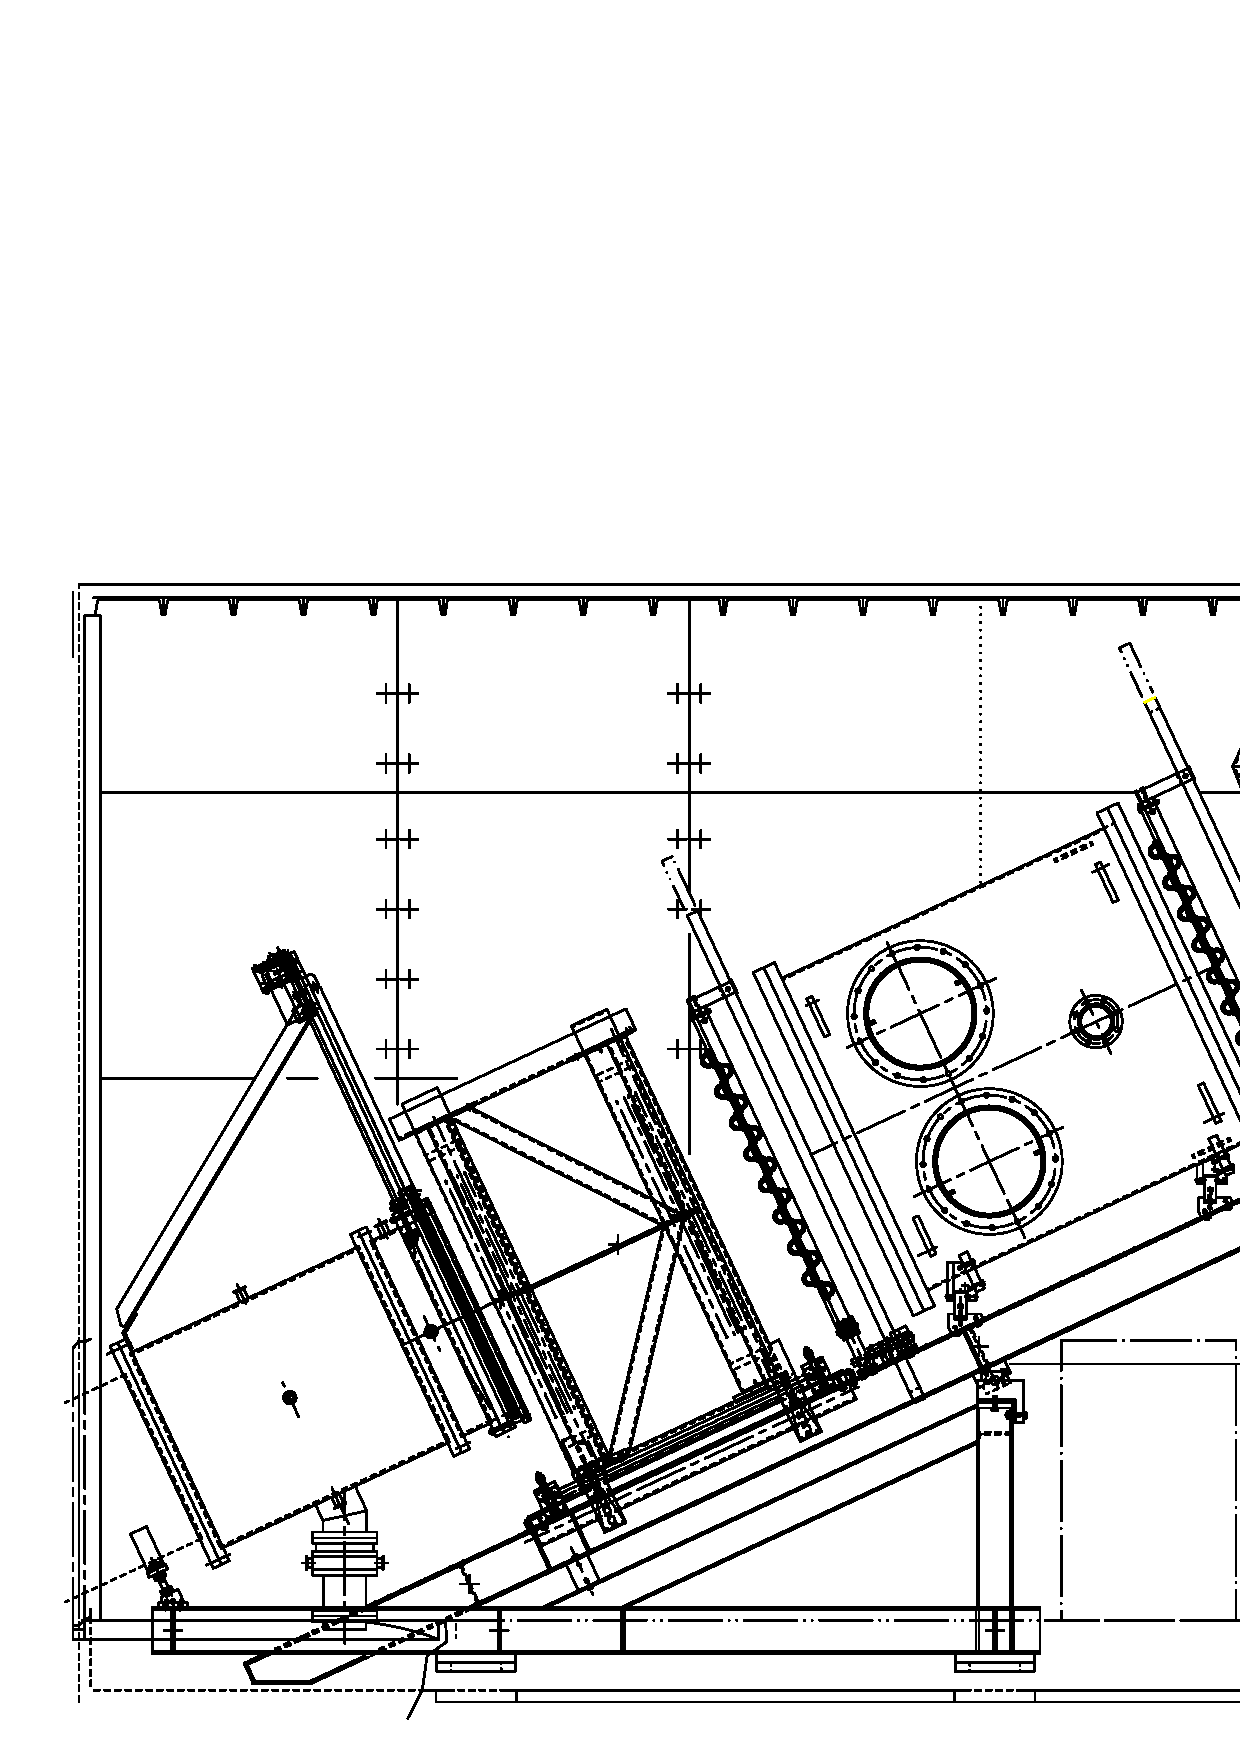
\includegraphics[width=4in]{figHMShut}
\caption{The HMS vacuum window in the HMS spectrometer hut. 
\label{fig:hms_window2}}
\end{center}
\end{figure}

\subsubsection{SHMS Windows}

The SHMS entrance window is on the front of the HB magnet. It has a rectangular shape.
The SHMS exit window is inside the Shield House detector room. It is mounted on the 
downstream end of the SHMS dipole when the Noble Gas Cerenkov (NGC)
is in use. Otherwise, it is mounted on the vacuum extension tank.  These two locations
are indicated in Fig.~\ref{fig:shms_exit_window_locations}.  Drawings of
the window and its flanges are shown in Fig.~\ref{fig:shms_exit_window}. When in use
the NGC provides protection for the vacuum window. When the window is placed on
the end of the vacuum extension tank, however, it must be protected by a roll-down
shutter that is interlocked with the detector-room door: if the door is open the shutter
must be down, protecting the window. Just like the HMS, \emph{the shutter needs to be
open when data is being taken by the SHMS, and the shutter may be opened only
after the shield door is closed.} The SHMS shutter controls are to be located near the 
exterior door of the SHMS shield house.

\begin{figure}
\begin{center}
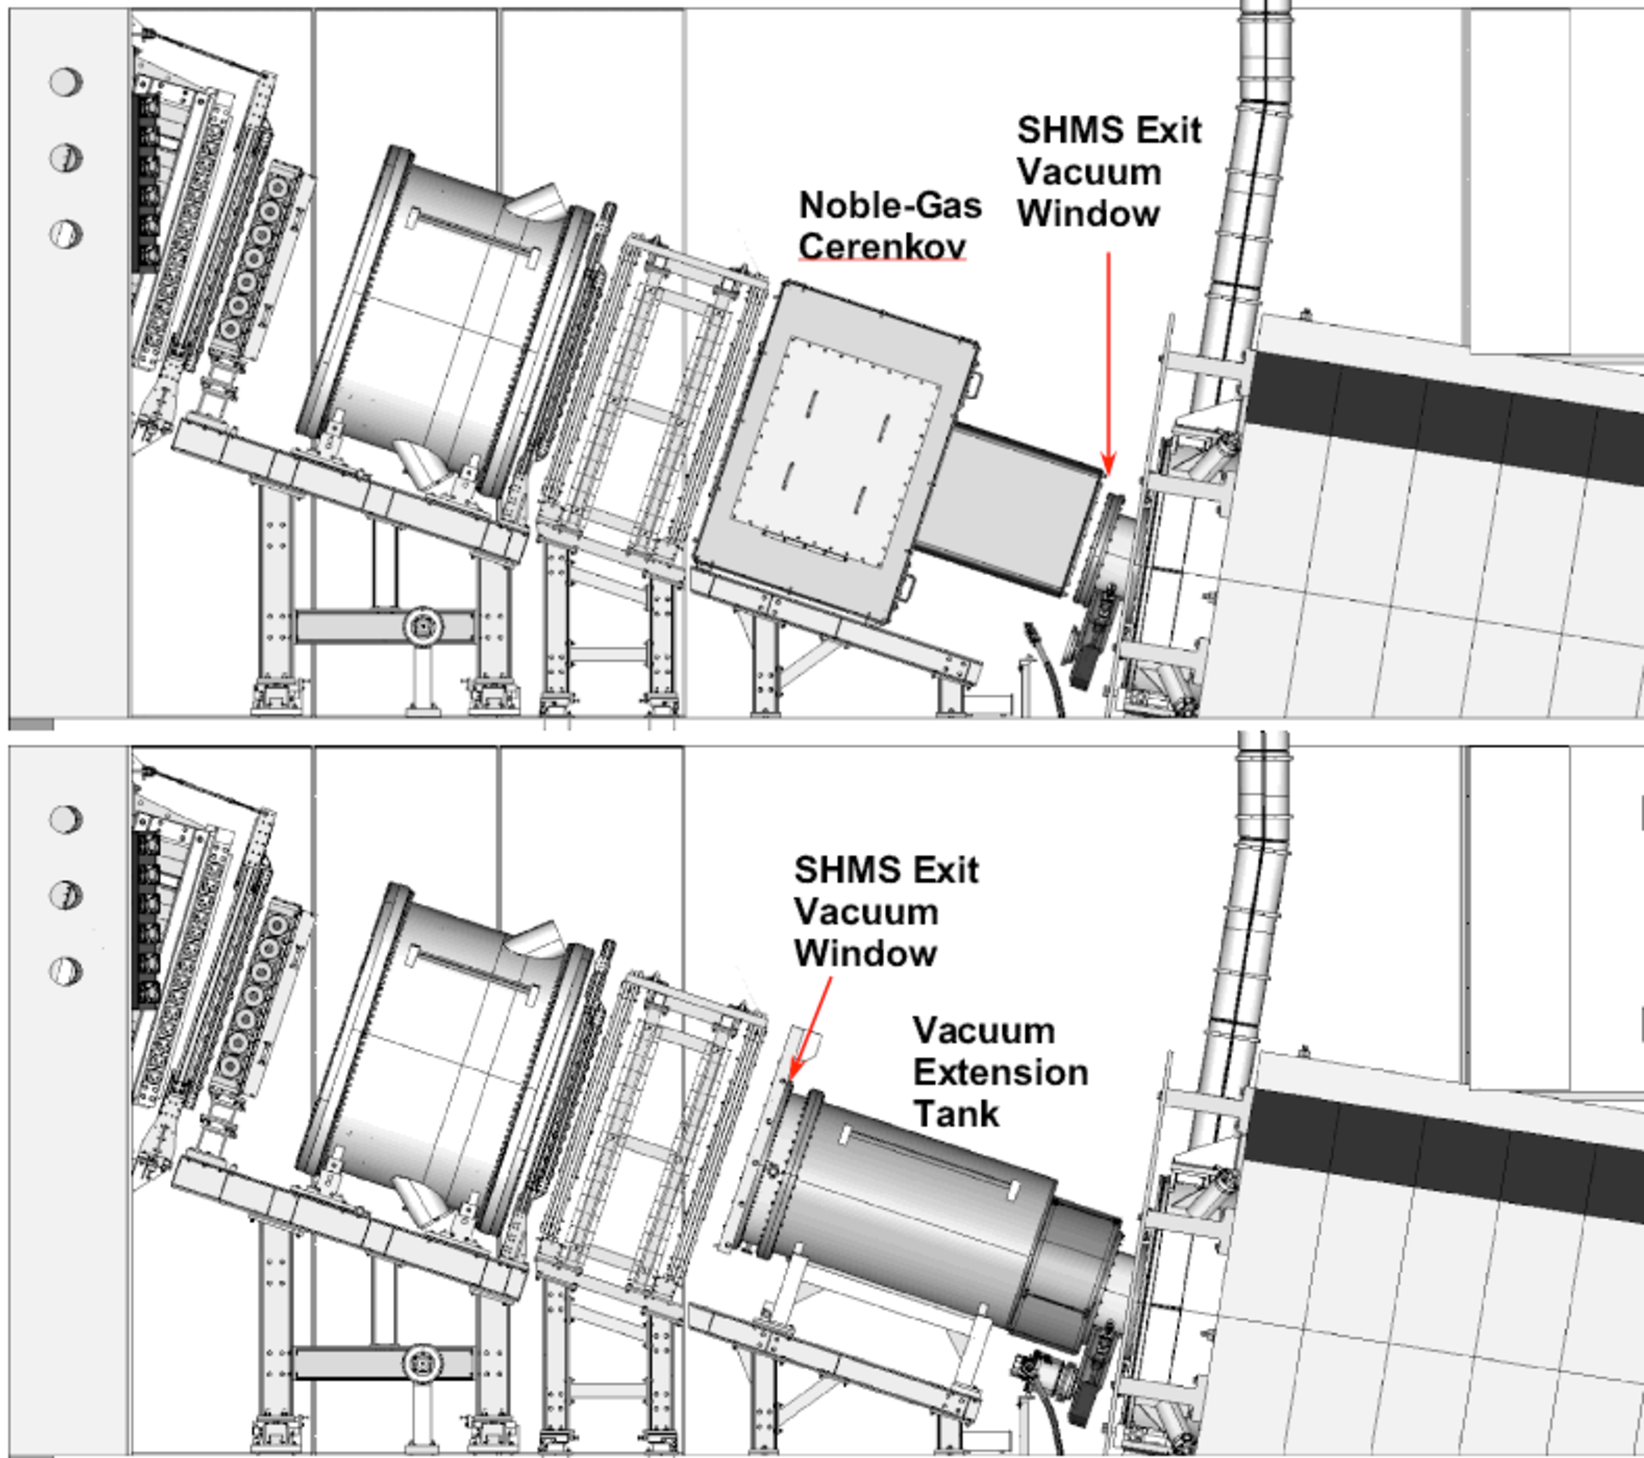
\includegraphics[width=6in]{figSHMS_ExitWindowLocations}
\caption{The two possible locations of the SHMS Exit Vacuum Window \label{fig:shms_exit_window_locations}}
\end{center}
\end{figure}

\begin{figure}
\begin{center}
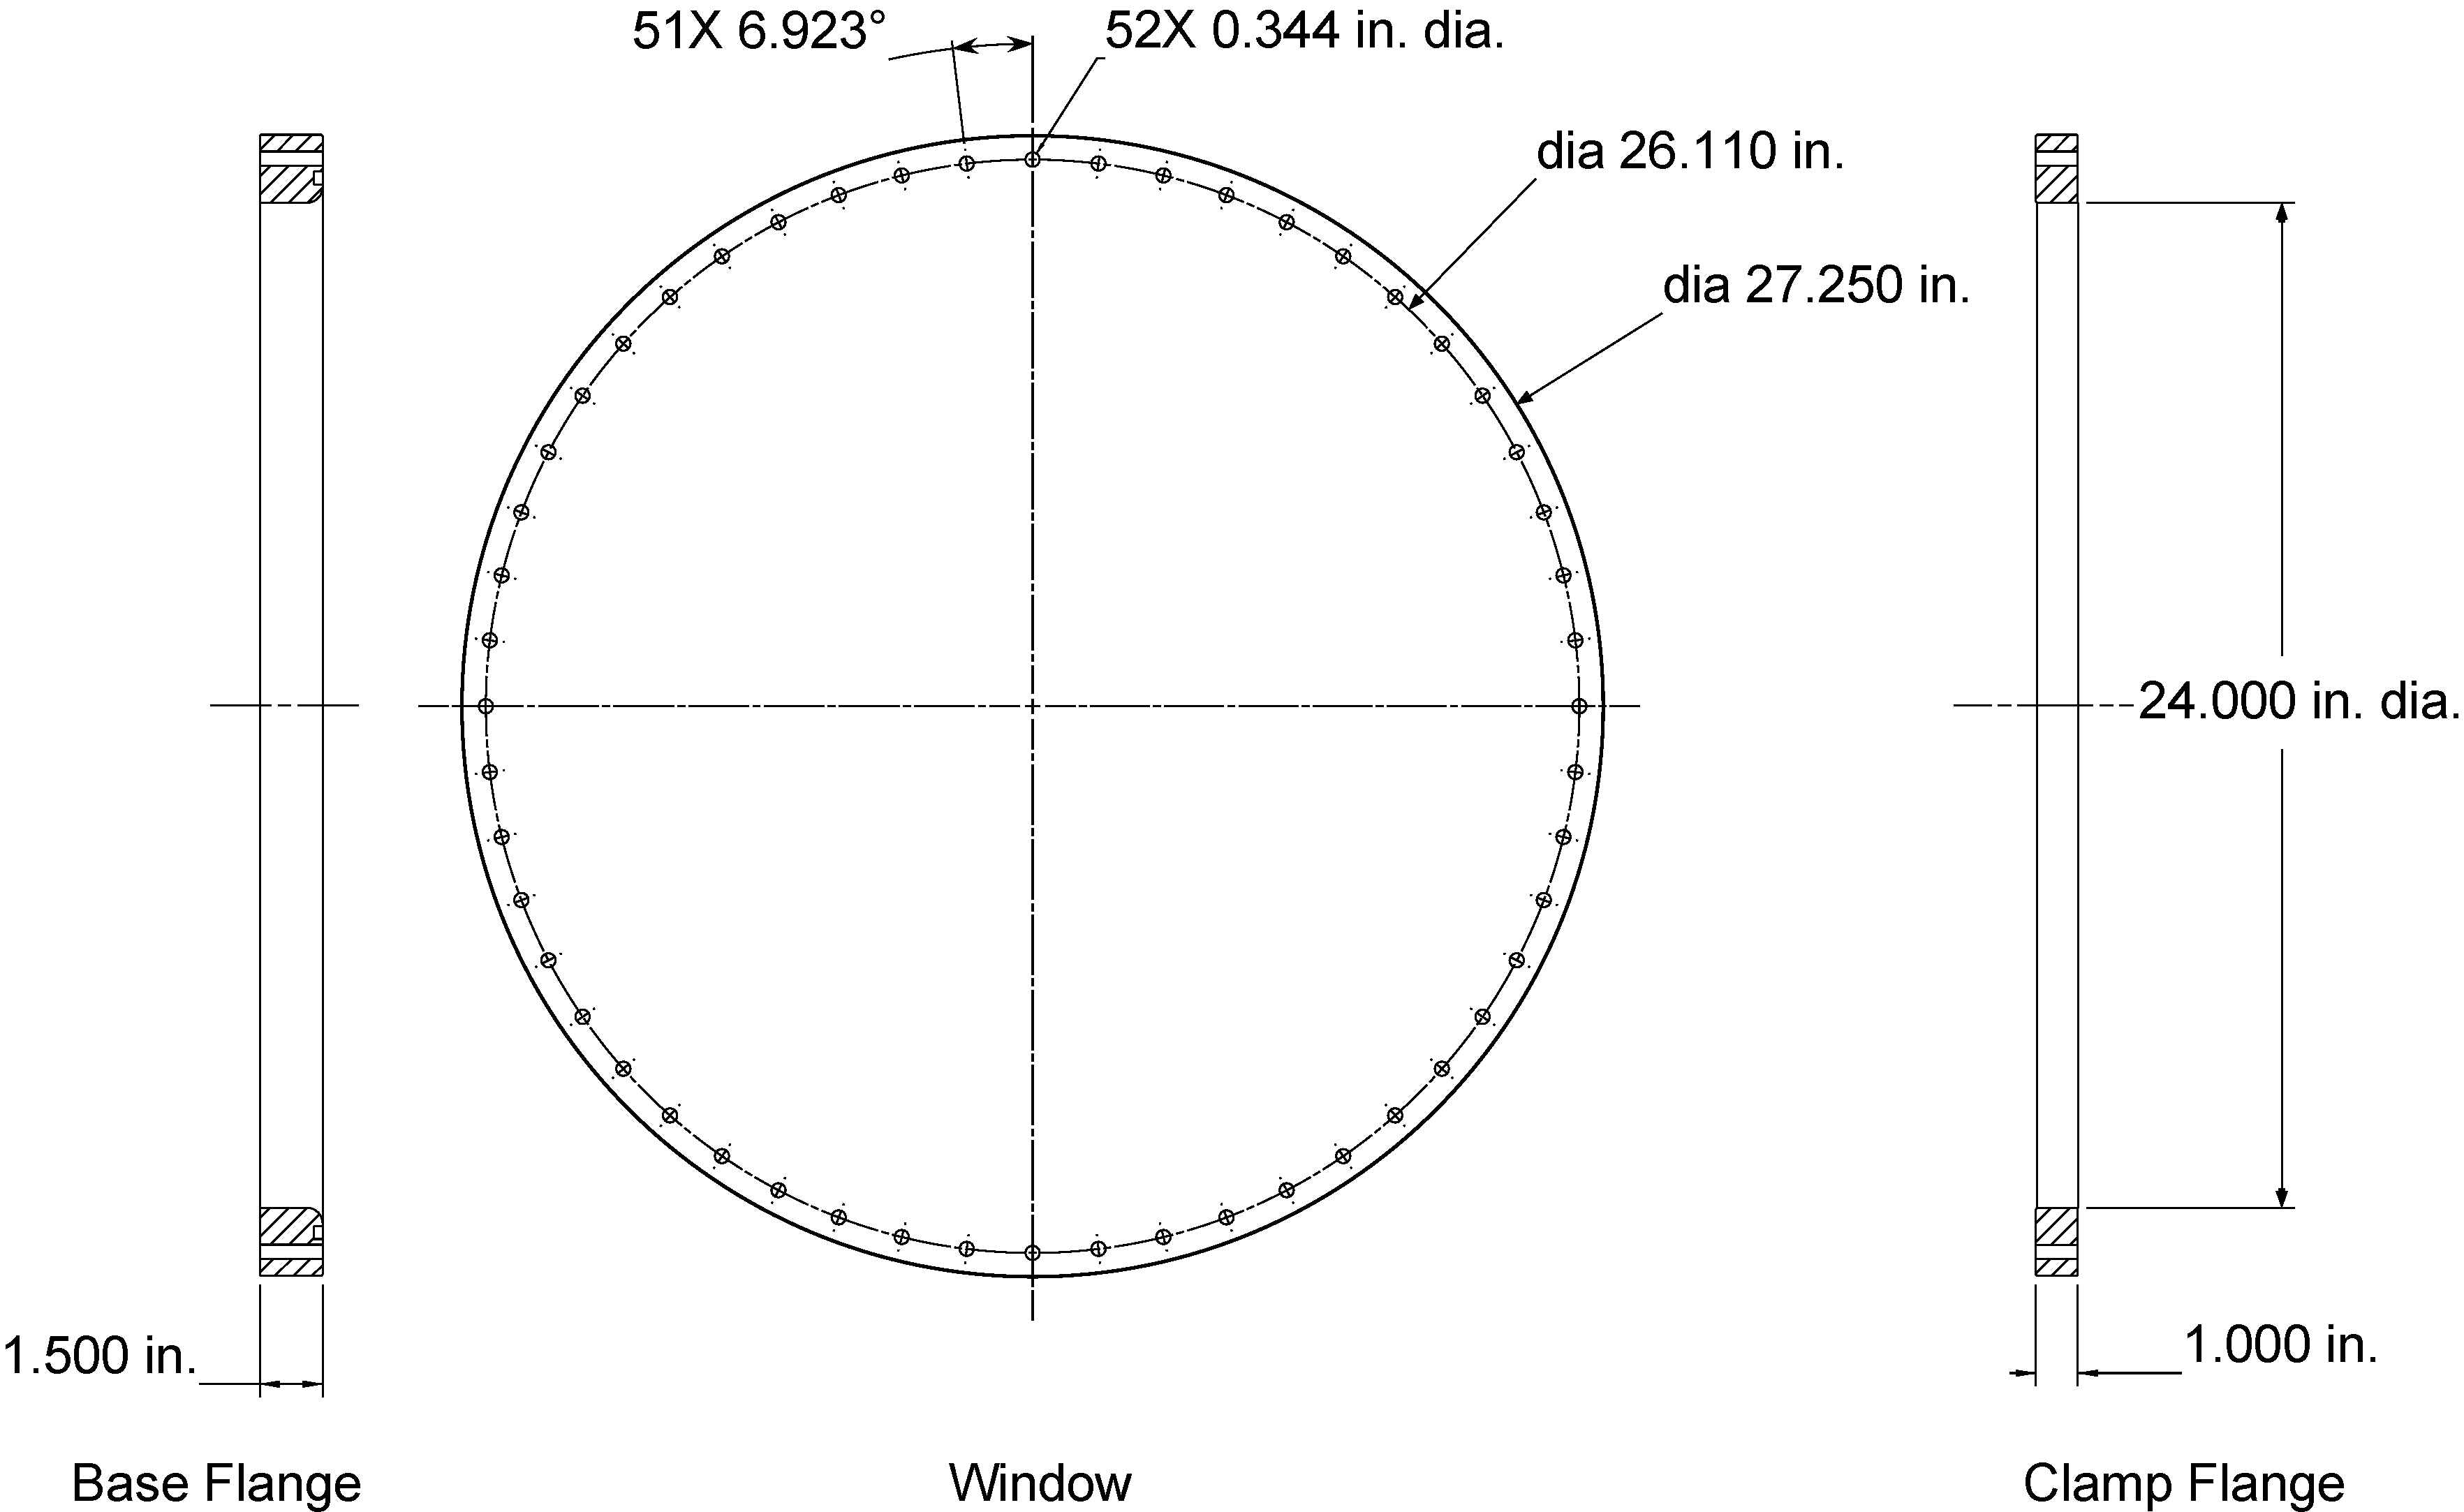
\includegraphics[width=4in]{figSHMSexitWindow}
\caption{The SHMS Exit Vacuum Window and Flange. \label{fig:shms_exit_window}}
\end{center}
\end{figure}

\section{Hall~C Spectrometer Magnets}

The basic parameters describing the magnets of the HMS and SHMS are provided in
Table~\ref{tab:magnet_parameters}. 

The quadrupoles determine the focusing properties of the spectrometers
and to a large extent their acceptance.
To achieve the lowest possible scattering-angle
settings for each spectrometer, both Q1's are
made asymmetric: narrow horizontally and elongated in the vertical direction. For the same
reason a notch is present in the outer mantles of both Q1 vacuum cans so
that the incident electron beam passes through this notch when the
spectrometer is at its smallest angle ($12.5^{\circ}$ for HMS and $5.5^{\circ}$ on the SHMS).

In order to reach such a small scattering angle, the SHMS is equipped with the HB
(horizontal bend) dipole magnet. It bends the central-ray tracks $3^{\circ}$ away from the
beamline so that the remainder of the spectrometer components are aligned $8.5^{\circ}$
from the beam when the spectrometer is rotated to center on a $5.5^{\circ}$ scattering angle.
When used at scattering angles below about $12^{\circ}$, the stray magnetic fields from 
the SHMS HB, Q1, and Q2 magnets can deflect the primary electron beam, possibly 
causing it to miss the beam dump, unless the schemes designed to prevent this are followed. 

The main dipole is the dispersive element in each spectrometer system. It 
determines the central momentum of the spectrometer.
The present operations envelope states that the HMS dipole power supply may not be
operated at currents above 1300 Amps. This corresponds to a central
momentum of about 4~GeV/c. 



\begin{table}
\begin{center}
\caption{Characteristics of the SHMS Magnets\label{tab:magnet_parameters}}
%\vspace{\baselineskip}
\resizebox{\textwidth}{!}{%
\begin{tabular}{|l|c|c|c|c|c|r|r|r|r|} 
\hline
		&		&		&			&\multicolumn{4}{|c|}{Values at Maximum Momentum}		\\
		&     		& Eff. Len.	& Aperture	&\multicolumn{1}{|c|}{Mom.}	&\multicolumn{1}{|c|}{Current}	&\multicolumn{1}{|c|}{Field or}	&\multicolumn{1}{|c|}{Energy}\\ 
		&     		&(m)		& (cm)		&\multicolumn{1}{|c|}{(GeV/c).}	&\multicolumn{1}{|c|}{(A)}		&\multicolumn{1}{|c|}{Gradient}	&\multicolumn{1}{|c|}{(MJ)}\\ 
\hline
HMS Q1	& Cold Iron	& 1.89	& $\phi~40$	&4		& 580	&1.25~T	& Asked	\\ 
HMS Q2	& Cold Iron	& 2.10	& $\phi~60$	&4		& 440	&0.3~T	& Fowler to\\ 
HMS Q3	& Cold Iron	& 2.10	& $\phi~60$	&4		& 220	&0.65~T	& provide	\\ 
HMS D	& Wam Iron	& 5.26	& $42 (w)$	&4		&1300	&1.11~T	& 7/27/16	\\ \hline

SHMS HB	& ``C" Septum	& 0.752	& $14.5 \times 18$	&11	& 3930	&2.56~T	& 0.2		\\ 
SHMS Q1	& Cold Fe		& 1.86	& $\phi~40$	&11		&2455	&7.9~T/m	& 0.39	\\ 
SHMS Q2	& $cos(2\theta )$& 1.64	& $\phi~60$	&11		&3630	&11.8~T/m& 7.6	\\ 
SHMS Q3	& $cos(2\theta )$& 1.64	& $\phi~60$	&11		&2480	&7.9~T/m	& 3.4	\\ 
SHMS D	& $cos(\theta )$& 2.85	& $\phi~60$	&11		&3270	&3.9~T	& 13.7	\\ \hline
\end{tabular}
}
\end{center}
\end{table}

\subsection {Magnet Cryogenics}

The HMS and SHMS magnets are all
superconducting and hence their coils must be maintained at
cryogenic temperatures during operations. The LHe required by the magnets
is supplied by the End Station Refrigerator, ESR.
All of the spectrometer cryogenic services are supplied through the overhead
cryogenic lines. The distribution network begins at the distribution
box over the pivot. This box is connected to the HMS and SHMS networks via the
flexible transfer lines over the pivot. The network is adjacent to
the upstairs catwalk on the HMS and, on the SHMS, is along the small-angle side
of the upper platform.

Cryogenic information about each magnet is available on the control
screens located in the Hall~C counting house.

All of the magnets were originally designed to be cryostable, meaning that they
cannot quench unless the level of liquid helium drops below the coils. Testing of
the HMS magnets up to their 4~GeV/c settings has shown that this design goal
was achieved. Nevertheless, the energy stored in the field of each magnet is sufficient 
to cause an unrecoverable quench if all of it were dumped into the magnet. 
Therefore, every superconducting spectrometer magnet in Hall~C, even though 
cryostable, is protected by a quench protection circuit. This circuit safely dissipates
much of the magnetic-field energy in a high-power dump resistor. The SHMS
magnets have not received extensive cryostability testing yet. 

\subsection {Magnet Power Supplies}

The power supplies for the magnets are located on the carriage
adjacent to the magnets. The supplies are all water cooled and
the water flow rate to the supplies can be seen on the water flow
meter located near the electronics boxes on the floor near the pivot.
This meter views the flow for all the HMS power supplies
(dipole and quads) and a reading of 33 $\%$ corresponds to approximately
20 gallons per minute through the combination of supplies (they are supplied
in parallel).
As of writing, the total flow rate for the SHMS power supplies has not been 
measured. When it is measured, the nominal value will be available in the Hall-C electronic log book
and the manual you are reading will be updated. 

The front panels of the power supplies are interlocked. Under
no circumstances should the front panel of any supply be opened by anyone other
than authorized personnel.

When the supplies are energized there are flashing red lights  and 
illuminated "Magnet On" signs placed at
several locations on the HMS and SHMS carriages to alert personnel to the magnet
status. There are also signs posted listing the dangers of high magnetic
fields.

The control interfaces for the power supplies are available in the 
Hall~C counting house on the HMS and SHMS control screens. Experimenters
use these screens to control the magnet power supplies. The magnet experts
will sometimes use controls that are local to the power supplies.

\subsection {Magnet Personnel}
In the event that any problems arise during operations of the magnets
of either the HMS or the SHMS,
one of the qualified responsible personnel listed in 
Table~\ref{tab:spec:personnel_magnet} should be consulted.  This includes any prolonged
or serious problem with the source of magnet cryogens (the ESR).
On the weekend and after hours there
will be a designated individual on call for magnet services. This person should be
contacted first. 


%\subsection{Quadrupole Magnets}
%
%The quadrupoles determine the transverse focusing properties of the spectrometers
%and to a large extent their acceptance.
%
%All three quadrupoles for the HMS spectrometer are cold iron superconducting
%magnets. The soft iron around the superconducting coil enhances the field at
%the coil center and reduces stray fields.
%The basic parameters for the first quadrupole, Q1, are an effective (actual)
%length of 1.89 (2.34) meter and an inner pole radius of
%25.0 centimeter. \cite{bi:yan1}
%The vacuum vessel
%inner radius for Q1 is 20.05 cm. To achieve the lowest possible angle
%setting of the HMS spectrometer (with respect to the beam line), Q1 is
%made asymmetrical, and is elongated in the vertical direction. For the same
%reason a notch in the outer mantle of the Q1 cryo vessel is made, such
%that the incident electron beam passes through this notch when the
%HMS spectrometer is at its smallest angle of 12.5 degrees.
%The other two quadrupoles, Q2 and Q3, are essentially identical with an
%effective (actual) length of about 2.10 (2.60) meter and an inner pole radius
%of 35.0 centimeter. For these quadrupoles the vacuum vessel inner radius
%amounts to 30.0 centimeter.
%
%% These will need to be updated for whatever max momentum we certify
%The maximum operating currents (assuming a 4 GeV/c momentum particle) for the
%quadrupoles are about 580 A, 440 A, and 220 A, for Q1, Q2, and Q3, respectively.
%To establish a correct focusing onto the detector plane with
%the quadrupole triplet we may want to cycle the quadrupoles to about 20\% higher
%current values, rendering maximum currents of 700 A, 530 A, and 270 A,
%respectively. This will render pole field values of 1.25, 1.30, and 0.65 T,
%respectively.
%The energy stored in the quadrupole fields is sufficient to cause an
%unrecoverable quench if all the energy stored is dumped into the
%magnets. \cite{bi:hms1}
%Therefore a quench protection circuit is incorporated. However, a quench
%can only happen if the cryomagnets have a helium level below the coil during
%operation.
%
%The operating current to the quadrupole coils is provided by three
%Danfysik System 8000 power supplies, which can operate up to 1250 A current
%and 5 V voltage. The power supplies are cooled with a combined maximum 
%water flow of 45 liters per minute.
%
%In addition to the main quadrupole windings, all quadrupoles have multipole
%windings to make corrections to the fields.  These mulitpole windings
%are no longer used and are not connected to power supplies.
%%To further optimize focusing properties of the HMS magnet system
%%we may operate some of these multipole trim coils
%%\cite{bi:yan2}.
%%The operating current for these multipole
%%corrections is small (the multipole corrections are typically less than
%%2\% of the main quadrupole field), of order 50 A, and are provided by
%%three HP power supplies. These power supplies can operate up to 100 A current
%%and 5 V voltage.
%
%%%
%
%\newpage
%\subsection{Dipole Magnet }
%
%The dipole is the dispersive element in the system and 
%determines the central momentum of the spectrometer.
%The present operations envelope states that the supply may not be
%operated at currents above 1300 Amps. This corresponds to a central
%momentum of $\approx$4 GeV/c.
%
%The dipole for the HMS spectrometer is a superconducting, cryostable magnet.
%Its basic parameters are an effective length of 5.26 meter,
%a bend radius of 12.06 meter, and a gap width of 42 cm.
%Its actual size is 5.99 meter long, 2.75 meter wide, and 4.46 meter high.
%It is configured to achieve a 25 degree bending angle for 4 GeV/c momentum
%particles at a central field excitation of 1.11 T.
%For the HMS dipole to reach 1.11 T the maximum operating current for the coil
%amounts to 1300 A.
%
%The dipole has been designed to achieve cryostability up to a field of 2 T,
%and this property has been extensively tested up to a field of 1.11 T.
%The cryostable coils are equipped with an energy removal circuit to cover
%the possibility of an unrecoverable quench. \cite{bi:hms2}
%However, this can only happen
%if the helium level drops below the coil during operation.
%The current to the coils will be provided by a Danfysik System 8000 power
%supply, which can operate up to 3000 A current and 10 V voltage.
%This power supply is located on the carriage beside the dipole, and
%is cooled with a maximum water flow of 35 liters per minute.
%The flow of the magnet cooling water is regulated by flow meters installed
%on the floor of Hall~C. The total water flow needed to cool the 4 power
%supplies for the HMS magnet system (dipole and quadrupoles) amounts
%to 80 liters per minute, with a supply pressure of cooling water for
%Hall~C of 250 psi.


\subsection{Operation of the Spectrometer Magnets \label{ssec:operatemagnets}}

HMS and SHMS magnet controls have been extensively revised. See section
\textbf{5.9 Superconducting Magnet Controls} for instructions. The controls and
monitoring screens are accessed through a GUI/HMI that magnet system 
experts will have initialized in the Counting Room. 

The information immediately following is being temporarily retained and is likely
covered in more detail elsewhere.

\subsubsection{Setting Magnet Currents}

The polarities of the currents in the HMS and SHMS magnets are such that
HB, Q2 and DIPOLE have the same sign as the charge of the particles
to be transmitted. Q1 and Q3 have the other sign. If you use the ``standard
tune" setting on the controls GUI this will be handled for you automatically.

While in the past users of Hall~C had to run a program called ``field" to obtain
the predicted current or field settings for a given spectrometer momentum,
these parameters are now determined for you by the controls program. You
need only to enter the desired momentum in the GUI.

One thing has not changed:
\begin{itemize}
\item{Wait at least 7 minutes for the HMS dipole magnet to settle.}
\end{itemize}

Up to this moment we have not witnessed any clear signature of hysteresis
effects for the HMS dipole magnet. For the HMS quadrupole magnets a small effect
on the field has been witnessed, but only for low currents (typically smaller
than 100 A). A procedure for setting the quadrupoles was developed
and shown to achieve a high
degree of reproducibility in setting the quads at low current.  
\\
\\
\textbf{The HMS Quadrupole Cycling Procedure:} 
\begin{enumerate}
  \item{On every change of polarity, take the magnet up to 950 Amps 
     (in the new polarity!), then down to zero before setting the
     current.} 
  \item{To set the current the first time after a polarity change 
     go up to 200 Amps higher than the desired current, 
     then down to the desired current.

     This means: to change the polarity and set the current go to 950 Amps,
     down to zero, back up to 950 Amps, and down to the desired setting.}
  \item{Subsequently:
  \begin{itemize}
     \item{Changes to lower currents can be made directly. 
        That is, just set the magnet for the lower current.}
     \item{For changes to higher current, first overshoot 
        by 200 Amps, then come back down to the desired current.}
  \end{itemize}}
\end{enumerate} 
This procedure is called \textbf{CYCLING THE MAGNET}, and needs to be  followed for all three HMS quadrupoles.

Commissioning of the SHMS magnets has not occurred as this is written, although it
is expected that only SHMS Q1 might need to by cycled. The other SHMS magnets have
current-dominated fields (rather than iron-dominated) and are not expected to 
exhibit significant hysteresis effects. Cycling procedures, if needed, will be established by
the Physics Division Liaison in consultation with the engineering group and collaborators.

\subsubsection{Checking Cryogenics}

\begin{description}
\item{\bf 1}\hskip0.1in Routine checking
\item{}\hskip0.3in The HMS and SHMS magnets all operate with liquid-level controlled
reservoirs. It is therefore sufficient to verify that the liquid level
is near the set point to be assured of cryogenic happiness.
\end{description}

\begin{description}
\item{}\hskip0.3in The setpoints are all 70\%.  The liquid
level is normally within a few percent of this value.  If
the helium level is significantly above this
the helium reservoirs are overfilling.  This is not harmful and the
levels will return to normal in several hours.  If the level is
significantly below the set points (5\% or more) there is usually
something wrong.  Selecting a time graph of liquid level is helpful in
determining if the situation is a temporary fluctuation or if the
situation is serious.
\item{\bf 2}\hskip0.1in Helium Problem Resolution
\item{}\hskip0.3in If helium liquid level is observed falling, check the cryogen status of all nine magnet
systems.  If multiple systems are losing liquid helium,  call CHL x7405 as the
likely cause is a site wide problem.  CHL will advise if recovery is
short (1-2 hours) or much longer.  If the recovery is short do nothing!
If the recovery is long then it can be beneficial to make some
adjustments in Hall~C.  This requires an access and a knowledgeable
individual: the on-call Hall~C magnet responsible person
should be summoned. Refer to Table~\ref{tab:spec:personnel_magnet}.
\item{\bf 3}\hskip0.1in Single System Failures
\item{\bf 3.1}\hskip0.1in Single System Loss of LN$_2$
\item{}\hskip0.3in If a single system is observed losing LN$_2$ you can
wait until
the next day to call someone in as the LN$_2$ usage of all the magnets
is extremely low.  They can go for 24 hours without a refill. Remember that the
HB magnet on the SHMS uses no LN2, so do not let that confuse you.
\item{\bf 3.2}\hskip0.1in Single System Loss of LHE Level
\item{}\hskip0.3in This is usually caused by a single computer failure or
components failure.  Call the on-call magnet responsible person (Table \ref{tab:spec:personnel_magnet})
and plan an access to Hall~C. The dipole reservoir will go empty in 1 hour so a quick reaction is
necessary.  The quads take much longer, 4 hours or more to empty
allowing more time to react.  All of the magnets have low level
interlocks that will automatically safely discharge the magnets 
so that you can safely operate until they are ``dry."
\item{\bf 4}\hskip0.1in Temporary Loss of LN$_2$ To All Systems
\item{}\hskip0.3in Occasionally during site LN$_2$ delivery, the supply to
Hall~C
is temporarily stopped.  This can be checked by calling CHL@7405.  There
can be local Hall~C problems that result in loss of LN$_2$ to the
magnets. The ``call in" can be deferred to a convenient time for this
kind of problem.
\end{description}
%
%\begin{table}
%\begin{center}
%\caption{Current Liquid Level Settings\label{tab:liq_levels}}
%\vspace{\baselineskip}
%\begin{tabular}{|l|l|l|}
%\hline
%{} & {}  & {}  \\
%{} & LHE & LN2 \\
%{} & {}  & {}  \\ \hline
%Q1  & 75\% & 75\% \\
%Q2  & 75\% & 75\% \\
%Q3  & 75\% & 75\% \\
%Dipole& 70\% & 70\%/65\% (Hi/Low) \\
%\hline
%\end{tabular}
%\end{center}
%\end{table}
%

\section{Spectrometer Vacuum Systems}

	Each spectrometer contains several separate vacuum volumes.
These are the isolation vacuums of each of the superconducting
magnets and the main spectrometer volumes through which the particles
to be detected travel.

The isolation vacuums are normally cryo-pumped by the cold mass when the
magnets are cold and hence have no mechanical pumps
associated with their maintenance. They also have no thin
windows or other hazards and will not be discussed further in this document.

The main spectrometer vacuum of the HMS
is maintained by the two mechanical pumps.
One pump is located between Q3 and the Dipole on the small angle
side of the carriage while the second pump is the backing
pump of the turbo. It pumps the spectrometer volume through the turbo.
This mechanical pump is located
at the back of the carriage and the turbo is located in the shield house
underneath the end of the vacuum can that protrudes into the detector hut.
The vacuum in the HMS channel may be read out on a gauge that is sitting on the
carriage beneath Q3. There is a TV camera that views this gauge readout and
it is displayed on one of the TV monitors  in the Hall~C counting house. 

A similar installation creates the vacuum in the SHMS channel. The mechanical
pump sits on the beamline-side of the SHMS carriage below the
upstream end of the dipole magnet. It is connected to the vacuum channel
through a port on the bottom of the plenum on the downstream end of the
dipole, inside the shield house. The vacuum level is monitored by the
readout included on the SHMS controls GUI.

If either spectrometer vacuum starts to deteriorate rapidly an expert should be notified.
Vacuum system responsible personnel are listed in Table ~\ref{tab:spectrometers:personnel_vacuum}.



\section{Spectrometer Slit Systems}
\label{sec:hms_slit}

The HMS slit system is installed on the gate valve housing mounted to the
front face of Q1. It consists of a vacuum box with a slit ladder
mounted into it. The slit ladder has space for three separate slits,
which will typically be one sieve slit and two solid angle defining collimators.
The slits are rectangular blocks of densimet (90\% W and 10\% Cu/Ni)
with a density of 17 g/cm$^3$. The collimators have an octagonal shaped
opening machined into them; the sieve slit has many holes drilled
into it.

The outer size of the collimators is 11.75" vertical by 8.25"
horizontal. The outer size of the sieve slit is 10.00" vertical
by 8.25" horizontal.
Its vertical size is reduced w.r.t. 11.75" due to space constraints.
The sieve slit always has to be installed at the bottom position of the ladder,
so that we can use the shielding of the collimator above it to
clearly distinguish the top row of holes. The central hole
of the sieve slit has a smaller aperture, and two blocked holes
exist to easily distinguish center and directions.
The collimator thicknesses are 2.5", while the sieve slit thickness
is 1.25". The dimensions and shape of the inner aperture of the present
HMS collimators is denoted in Table~\ref{tab:apertures}.

\begin{table}
\begin{center}
\caption{Apertures of Collimators\label{tab:apertures}}
%\vspace{\baselineskip}
\begin{tabular}{|c|c|c|c|c|c|}
\hline
{} & {} & {} & {} & {} & {} \\
HMS				& d$\Omega$ 	& Horizontal 	& Vertical 		& Shape 			& Note \\
{} 				& (msr) 		& (mr) 		& (mr) 		& {} 				& {} \\
{} & {} & {} & {} & {} & {} \\ \hline
{}Need Description	& 6.74 		& $\pm$ 27.5 	& $\pm$ 70.0 	& Octagonal, Flared 	& Quads Nominal \\
{}	 			& 6.74 		& $\pm$ 27.5 	& $\pm$ 70.0 	& Octagonal, Flared 	& Quads Backward \\
{} & {} & {} & {} & {} & {} \\ \hline
%SOS & 7.55 & $\pm$ 57.5 & $\pm$ 37.5 & Octagonal, Flared & \\
%SOS & 3.98 & $\pm$ 32.5 & $\pm$ 35.0 & Octagonal, Flared & \\
SHMS			& d$\Omega$ 	& Horizontal 	& Vertical 		& Shape 			& Note \\
{} 				& (msr) 		& (mr) 		& (mr) 		& {} 				& {} \\
\hline
\end{tabular}
\end{center}
\end{table}

The total depth of the slit box is close to 3.75", which leaves
enough space to later mount scintillators behind the collimators as an active
veto counter (to prevent punch-through of hadrons) and/or to increase
the collimator thickness. Two circular quick-connect flanges are
added for feed-through of possible light guides.

A similar remotely-operated collimator box is installed on the SHMS between the
HB and Q1 magnets. The collimator ladder assembly within this box may be positioned
at three settings. The top position (accessed when the assembly is at its lowest
position) is a stretched octagon with opening height 9.843" and width 6.693" on the
upstream side. It is 2.5" thick. The lower two positions both present sieve holes in
rectangular pattern with holes separated by 0.6457" horizontally and 0.9843"
vertically. The sieve pattern at the middle ladder position has 11 columns of holes with
the sixth column centered horizontally. The holes on the bottom sieve are in ten
columns and are offset by one-half a column gap from those in the middle sieve.
The sieve collimators are 1.25" thick. The geometry is illustrated in Fig.~\ref{fig:SHMS_Collimators}.
Both sieves and octagonal collimator are
made of Mi-Tech\texttrademark{} Tungsten HD-17 (Density 17 g/cc. 90\%~W, 6\%~Ni, 4\%~Cu).

Because the SHMS has both a horizontal bend (HB magnet) and a vertical bend (main Dipole
magnet), a second sieve collimator is required for optics calibration. It is placed immediately
upstream of the HB magnet entrance. Two options are provided: a conventional passive
sieve collimator and the so-called \textit{active sieve} which is a detector based on Gas Electron 
Multipliers (GEMs).  A photo of the passive sieve options is shown in Fig.~\ref{fig:HB_Sieve_Photo}
and the dimensions and hole pattern are shown in Fig.~\ref{fig:HB_Sieve_Layout}.

\begin{figure}
\begin{center}
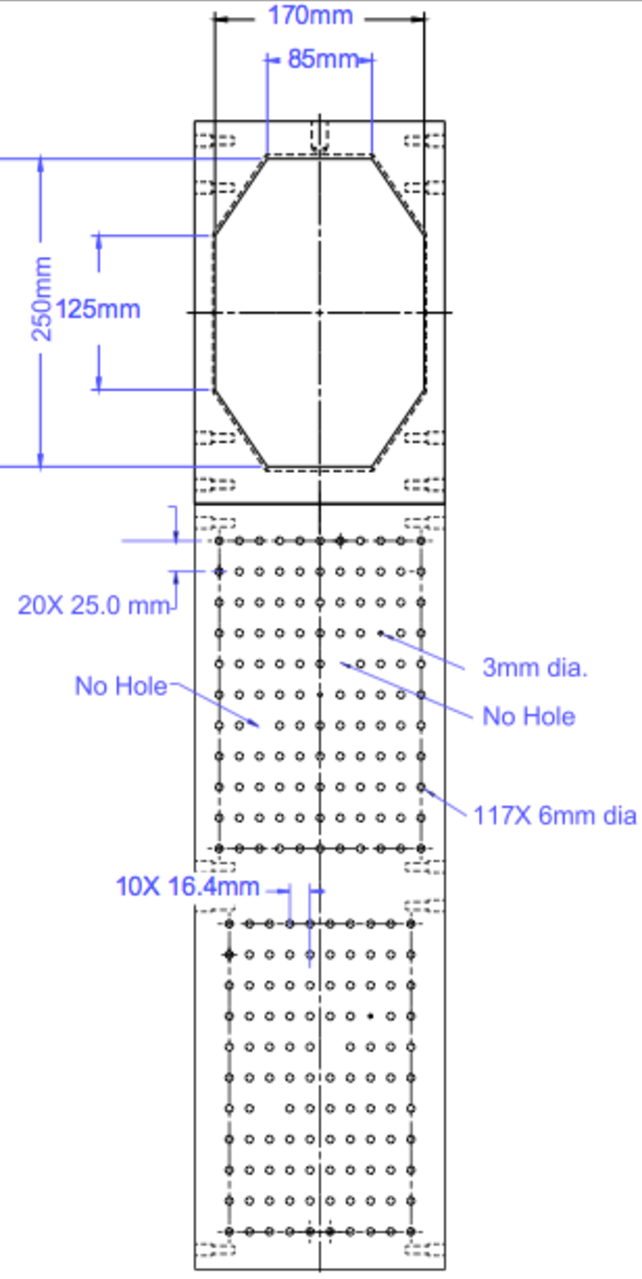
\includegraphics[width=2in]{SHMS_Collimators}
\caption{Geometry of the Main Collimator and the Sieve Slits in the SHMS \label{fig:SHMS_Collimators}}
\end{center}
\end{figure}

\begin{figure}
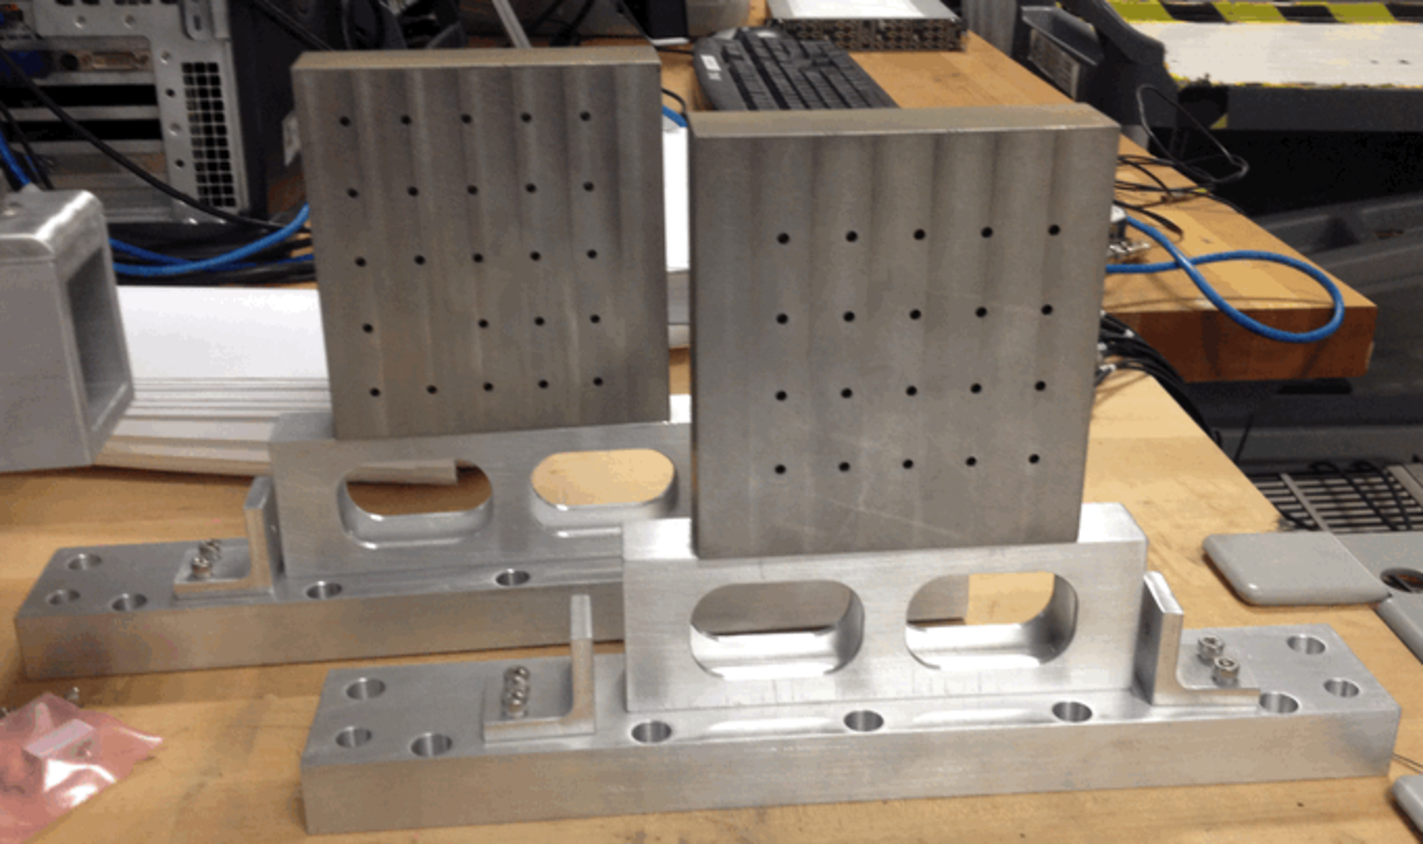
\includegraphics[width=6in]{HB_Sieve_Photo}
\caption{Upstream Sieve Slits that go on the front of the HB magnet of the SHMS \label{fig:HB_Sieve_Photo}}
\end{figure}

\begin{figure}
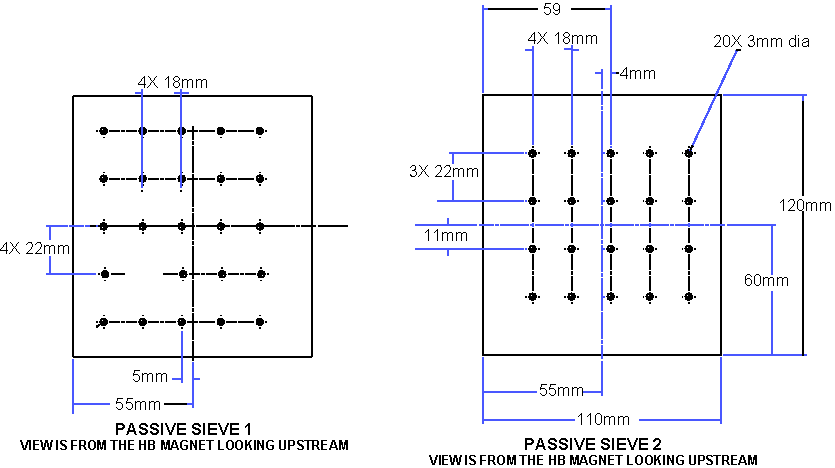
\includegraphics[width=6in]{HB_Sieve_Layout}
\caption{Upstream Sieve Slits that go on the front of the HB magnet of the SHMS \label{fig:HB_Sieve_Layout}}
\end{figure}

\subsection{Operation of the HMS Slit System}\label{sssec:slit_control}

{\bf IN 2016 EPICS DRIVERS AND SCREENS ARE BEING WRITTEN FOR 
THE COLLIMATOR MOTION CONTROLS. THE TEXT BELOW WILL NEED TO BE UPDATED.}

A remote control system consisting of motor/actuators exists to slide
the slits into place. Resolvers specify the exact position of the
slits.  The control box is located downstairs in Hall~C, behind the
blue power supply racks. On the front face there are four buttons for
each spectrometer. These indicate the three different slit positions
and the ``home" position, which denotes that no slit is used at all
(slit ladder in the up position).  Brake cables are added to prevent
the slit ladder from falling in case of a power loss. Next to this an
emergency button is included to electrically shut down the control
system.

{\bf After a power cycle the HMS slit moves itself to the {\it HOME} position,
returning a reading of 0. Thus, after a power failure or other cycle, the slit
must be commanded to a meaningful position using the commands described below.}


Normally, the system is operated remotely. Connect to the controller
using terminal server hctsv7, port 3:

\begin{minipage}{6in}
\begin{enumerate}
\item telnet hctsv7 2003
\item type \texttt{\\B} to connect to HMS, \texttt{\\A} for SOS. (Must be UPPER CASE)
\item {\tt P PFB} gives readback of the current position (see Table \ref{tab:col_pos})
\item To {\em MOVE} the collimators:
   \begin{itemize}
	\item {\tt EN} - to enable motion.
	\item {\tt RUN 10} - follow instructions (see slit numbers and postions at bottom)
	\item After you have reached the correct slit, disable the motor by typing {\tt 1}

   \end{itemize}
\item If necessary, \texttt{K} (kill) is the opposite of \texttt{EN}
\item Get rid of your session by typing \texttt{ctrl-]} (both pushed together), then
at the telnet prompt, type \texttt{quit}.
\end{enumerate}
\end{minipage}

Don't forget to get rid of your session. If you do not close your session nobody
else can communicate with the slit controllers.

%\begin{table}[!ht]\
%\caption{Slit Collimator Positions\label{tab:col_pos}}
%\begin{center}
%\begin{tabular}{rlrr}
%   &                  &     HMS   & SOS\\
%\hline
%1) & Sieve Slits      &  19804600 &  11638719\\
%2) & Large Collimator &       N/A &   3190717\\
%3) & Pion Collimator  &  -3096800 &       N/A\\
%\end{tabular}
%\end{center}
%\end{table}

\begin{table}[!ht]\
\caption{Slit Collimator Positions\label{tab:col_pos}}
\begin{center}
\begin{tabular}{rlrr}
   	&                  		&     HMS   	& SHMS			\\ \hline
1) 	& Sieve Slit 1   		&  19804600 	&  (Mark Jones)	\\
?) 	& Sieve Slit 2   		&       N/A 		&  (Mark Jones)	\\
2) 	& "Large" Collimator	&       N/A 		&  (Mark Jones)	\\
3) 	& "Pion" Collimator  	&  -3096800	&   N/A			\\
\end{tabular}
\end{center}
\end{table}

   
\subsection{Hazard Identification}

The principal hazards are:
\paragraph{Magnetic:} There is a significant fringe field at
the entrance and exits of the magnets. This represents a hazard
to people working on the slit system if they are handling magnetic
objects (tools) or to people with pacemakers. In addition the field could erase magnetic
information storage media such as the strips on credit cards.
\paragraph{Mechanical:} At the front of Q1 the housing for a spring loaded gate valve is
mounted. In its normal operation mode a metal gate will be closed with
severe pressure when the electrical power drops. This can cause serious
damage to interfering body parts.  But currently the shutter and
actuator have been removed so this hazard does not exist.  
A similar mechanical problem involves the slit ladder itself. The total weight of
the three slits amounts to approximately 350 Lbs (160 Kg) and can easily
cause serious damage to body parts.

\subsection{Hazard Mitigation}

\paragraph{Magnetic}

A sign will be posted which indicates the presence of a high magnetic
field ( this is standard JLab safety signage). The exact wording is
`` High Magnetic Field - No Pacemakers or Credit Cards." There are also
flashing red lights located on the HMS carriage indicating that the
magnet power supplies are energized. Be careful with tools (are they magnetic?)
when you work on the slit boxes with the red lights in a flashing state.

\paragraph{Mechanical}

If the gate valve is ever re-installed, the following safety
procedures should be observed.  Without power, the gate valve assumes its default closed position due to
pressured air. When installing the slit boxes, or working with your hands
in the vicinity of the inside of the gate valve, disconnect first the power
plug of the gate valve, such that the gate valve closes.
In case you need the gate valve to assume a default open position without
power, first relieve the air pressure
with power on, and verify that the default position of the gate valve has
changed to ``open" by removing the power. Paul Hood (x7849) or Mike Fowler
(x7162) can be contacted for more information.

When installing the slit ladder, be careful when you work with your hands
under the slit ladder (like when you are bolting the slit box to the
gate valve). Remove the slit ladder, or {\bf install a support under the slit
ladder to prevent it from falling all the way down}.

A brake system has been included in the control to prevent the slit ladder
from sliding down in case of a power failure.  However, this must not
be relied upon for personnel safety.


\section{Spectrometer Carriage and Rotation Systems}

The Carriage is the support structure of the spectrometer.

Each entire spectrometer can be rotated. Rotation is driven by motors mounted
near one of the sets of wheels. These motors are controlled by synchronous 
pulse width modulated drives which are mounted near the bottom of the shield 
house steps on the HMS, and under the rear of the SHMS structure.

The spectrometer angles are found using a reference plumb bob and/or TV camera
attached at a known location under the rear of each spectrometer.
This camera is focused on survey marks scribed into a plate which is attached to
the rail on the floor. Using the scribe plate and a vernier scale, the angle of the
spectrometer may be determined with a resolution of approximately $0.01^{\circ}$.

	
\begin{safetyen}{0}{0}
\subsection{Hazard Identification}
\paragraph{Spectrometer Rotation}

Movement of either spectrometer can cause serious damage if a person or 
object is in its way,
or is attached to it in such a way that it may be stretched, crushed, or dislodged. 
There is only a small gap between the rear of the SHMS shield house and the
shielding wall behind it. 

\paragraph{Hard Hats May be Required: Elevated Platforms:} 

Both spectrometer carriages are multi leveled structures. It is important to keep in
mind that people may be working above you.  Depending on working conditions, 
you may be required to wear a hard hat. 
Handrails are installed to prevent falls. Work only within the protected areas.

\paragraph{Magnetic:}

Any of the spectrometer magnets may be energized under either local or remote
control. When present, this hazard is indicated by either red flashing lights and/or
illuminated \textbf{Magnet on} signs. Keep out of any potential high-field zones.

\end{safetyen}

\subsection{Remote Rotation}

Prior to the start of experiment operations, Hall-C staff will certify that the spectrometers
are configured for safe remote rotation by verifying all required clearances and
implementing interlocks, mechanical stops, or administrative controls, as appropriate.
Refer to the section of this manual on \emph{Controls} to find instructions for
rotating the spectrometers. The cameras enable remote readout of the HMS/SHMS 
spectrometer angles using the survey marks on the floor.
The wide-lens and zoom cameras located at the entrance and
the exit of Hall~C should be used to visually search for obstructions
before and during remote rotation.

Limit switches are installed at forward
and backward angles which prevent HMS (SHMS) from rotating to angles more forward than
10.6 (5.5) degrees and wider than 85 (40) degrees. To obtain more forward or wider
angles an access is needed, and rotation has to occur manually
downstairs with spotters. Hard limit switches will be installed to prevent
the spectrometer from rotating out of maximum allowed range.

In case the spectrometers are rotated to more forward angles, pay special
attention to possible interferences of HMS and SHMS, and interference between either
spectrometer and the beam pipes or their stands. 

%Remote rotation  is accomplished via the PLC located in the Hall.  It
%is currently installed in the HMS shield hut for protection from
%radiation.  Commands can be issued to the PLC (Texas Instruments 5000), which executes these commands
%following algorithms stored in its memory. An EPICS screen is now
%used to talk to the PLC.  The advantages of using the PLC are:
%
%\begin{itemize}
%\item{No direct access by users to the algorithms, preventing unsafe
%rotation attempts (instead, the algorithms have to be loaded locally into
%the PLC).}
%\item{Rotation of both HMS and SOS by the same smart controller, enabling
%security checks of both angle decoders. This renders a better handle on the
%minimum allowed angle between the two spectrometers.}
%\item{Automatic slower rotation speeds (if desired) if close to desired angle
%when using proximity switches.}
%\end{itemize}
%
%The PLC communicates directly with the control electronics of several limit
%switches, proximity switches, and decoders. Next to the limit switches
%also hard limit switches will be installed on the floor to mitigate failure
%of the PLC limit switches.


\subsection{Personnel Trained for Manual Spectrometer Rotation}

The spectrometer motors may only be manually controlled by trained personnel. if it
is necessary to rotate the spectrometer manually, contact one of the trained
personnel listed in Table~\ref{tab:spectrometers:personnel_rotate}.
At least two people are required for manual spectrometer rotation: one to
run the motors and at least one spotter. Prior to rotating the spectrometer
a visual inspection of the area must be made to insure that there
is nothing in the spectrometer's path or on the rails. During rotation
the spotter should pay special attention to
the cables which run from the
spectrometer to the target motor controller to make sure that
nothing is hung up or stretching.

\begin{namestab}{tab:spectrometers:personnel_rotate}{Spectrometer Rotation: authorized personnel}{%
      List of Spectrometer Rotation responsible personnel where ``W.B.'' stands for the white board 
      in the counting house.}
   \TechonCall{\em Contact}
   \MikeFowler{}
   \WalterKellner{}
   \AndyKenyon{}
   \JoeBeaufait{}
\end{namestab}
}

%%%%%%%%%%%%%%%%%%%%%%%%%%%%%%%%%%%%%%%%%%%%%%%%%%%%%%%

\infoleveqnull{\section{Spectrometer Rotation}

\sawnote{This section is just for the ESAD.  Currently just based on the
Hall A ESAD.  The HMS rotation discussion above needs to be updated
and broadened to also include the SHMS and this ESAD text merged in.
Include statement that angle limits are set by experiment and that
movements to small angles may need to be done by experts.
}


%
%
Since the Hall C spectrometers each weigh in excess of \sawnote{XXX}
tons it is very important that all safety precautions are carefully
adhered to.   During operations, the spectrometers are certified
to allow remote rotation by shift crews within prescribed limits.  In
the absence of this certification, the spectrometers may only be
rotated by trained technical staff.

\begin{safetyen}{0}{0}
\subsection{Hazards}

Hazards include:
\begin{itemize}
\item{Knocking items over.}
\item{The wheels crushing things (including fingers and toes) on the floor in the path of the 
spectrometer}
\item{Damaging the beamline or other equipment on the floor if one goes to too small 
or too large an angle, or if it just gets pushed around inadvertently.}
\item{Tearing out of cables etc. physically attached to the superstructure}
\end{itemize}

\subsection{Mitigations}

Hazard mitigations:
\begin{itemize}
\item{Stop-blocks attached to the rails to prevent spectrometer rotation beyond the needed angular range.}
\item{Audible alarm on the spectrometers indicating they are in motion or that motion
is possible (controls engaged etc.)}
\item{During a running experiment the run coordinator and work coordinator should know in advance 
of any moves.  Moves at any other time must be cleared with the Hall work coordinator 
before implementation.}
\item{Careful inspection of the intended path to make sure it is clear. This is part of
the pre-run checklist performed by the technical staff prior to closing the Hall and
a remote camera allows shift worker to inspect the area.}
\item{Any motion that takes a spectrometer inside 14 degrees or outside \emph{X} degrees
(\emph{X} being specified in the pre-run checklist and noted on the whiteboard during a run) 
must be supervised by a trained Hall C technician.}
\end{itemize}
\end{safetyen}

\subsection{Responsible Personnel}

Following the experimental run plan, as posted in the counting house
by the run coordinator, shift workers are allowed to rotate the HRS
following guidelines of the standard equipment manual.  In the event
of a problem getting the spectrometers to rotate the run coordinator
should notified.  If the run coordinator is unable to solve the
problem, and with the run coordinators concurrence, qualified
personnel should be notified to repair the problem (see
Table~\ref{tab:spectrometers:personnel_rotate}).  On weekends and after hours
please only use the tech-on-call number.  It should be noted that for
experiments that are using thick targets at high current, it is not
uncommon that the produced radiation will cause the motion system to
require a hard reset.



}
